\section{Linear Programming}
\subsection{What's Linear Programming ?}
\begin{tcolorbox}[title = Definition] 
Linear programming is a sub-branch of optimization techniques. It involves modeling real-life problems as
linear equations and inequalities and using specialized methods to find optimal solution(s), if they exist.
\end{tcolorbox}
\vspace{1cm}
\begin{center}
    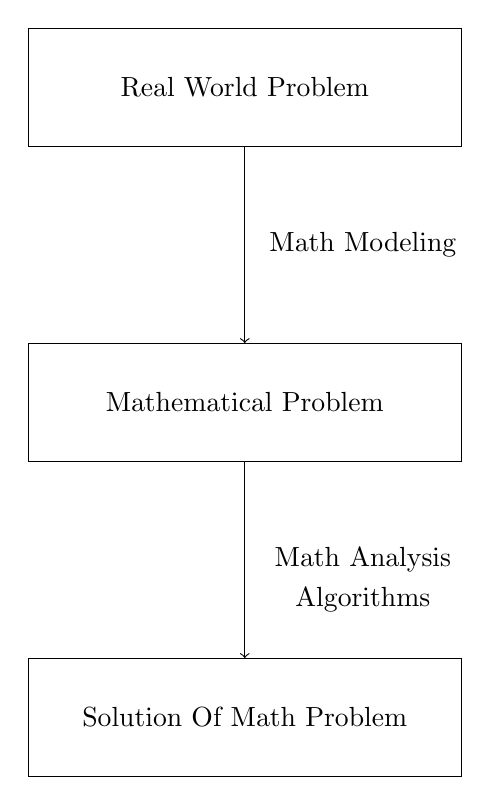
\begin{tikzpicture}
       \draw (0,0) rectangle (5.5,1.5);
       \node at (2.75,0.75) {Real World Problem};
      
       \draw[->] (2.75,0) -- (2.75,-2.5);
       \node at (4.25,-1.25) {Math Modeling};

       \draw (0,-4) rectangle (5.5,-2.5);
       \node at (2.75,-3.25) {Mathematical Problem};
      
       \draw[->] (2.75,-4) -- (2.75,-6.5);
       \node at (4.25,-5.25) {Math Analysis};
       \node at (4.25,-5.75) {Algorithms};
       
       \draw (0,-8) rectangle (5.5,-6.5);
       \node at (2.75,-7.25) {Solution Of Math Problem};
   \end{tikzpicture}
\end{center}
\vspace{1cm}
\subsection{Models}
\subsubsection{Graph Model}
This model is used when the objective function has two variables. It consists of converting all inequalities
into equalities, drawing them as lines, and then identifying the feasible area where all conditions are met.
We then sweep the objective function \(Z\) across the plot until we find the optimal solution(s).

\begin{tcolorbox}[title=Note]
 \textbf{\underline{Solutions : }}
When solving a linear program, the solution can be:
\begin{itemize}
    \item \textbf{One or Multiple Optimal Solutions}: The feasible area is a polygon, and its vertex points are the possible optimal solutions.
    \item \textbf{Infinitely Many Solutions}: If the solution is unbounded, then the objective function will increase or decrease infinitely as we sweep the line.
    \item \textbf{No Solution}: If the feasible area is empty (\{\(\emptyset\)\}), it indicates that the
system has contradictions.
\end{itemize}


\textbf{\underline{Direction of Increase/Decrease:}}

\begin{itemize}
    \item \textbf{Both Positive} \((a > 0\) , \(b > 0)\): Since both coefficients are positive, \( Z \) increases as
\( x_1 \) and \( x_2 \) increase, and decreases as they decrease. The direction of increase is towards the right,
and the direction of decrease is towards the left.

    \item \textbf{Both Negative} \((a < 0\) , \(b < 0)\): The opposite of the positive case. Here, \( Z \) increases
as \( x_1 \) and \( x_2 \) decrease, and decreases as they increase. The direction of increase is towards the left,
while the direction of decrease is towards the right.

    \item \textbf{Different Signs} \((a\) and \(b\) have opposite signs): The direction is determined by 
the coefficient with the larger absolute value, \(\max(|a|, |b|)\). If this coefficient is positive, the direction 
of increase follows the same pattern as when both coefficients are positive. If this coefficient is negative, 
the direction of increase follows the pattern for both negative coefficients.
\end{itemize}
\end{tcolorbox}



\subsubsection*{{\underline{Example1 :} Diet Problem}}

\vspace{0.25cm}
The Goal is to minimize food cost but to meet the minimum daily nutrition requirement
\vspace{1cm}
\begin{center}
\begin{tabular}{|c|c|c|c|c|c|}
    \hline
    Food & Units & Protein & Vit c & Iron & Price\\
    \hline
    Apples & 1 med & 0.4 & 6 & 0.4 & 8\\
    \hline
    Banana & 1 med & 1.2 & 10 & 0.6 & 10\\
    \hline
\end{tabular}
\end{center}

\newpage

\begin{multicols}{2}
\textbf{\underline{Variables Definition:}}\\

Let \(x_1\) be the number of Daily Unit Appels.\\

Let \(x_2\) be the number of Daily Unit Banana.\\
\columnbreak

\textbf{\underline{Constraint:}} 

\[
\left\{
    \begin{array}{l}
        \forall x_1 , x_2 \geq 0 \quad \text{(Non-negative number of food item) ...C1}\\
        0.4x_1 + 1.2x_2  \geq 70 \quad \text{(Minimum Protein Daily) ...\textcolor{greenPlot}{C2}}\\ 
        6x_1 + 10x_2  \geq 50 \quad \text{(Minimum Vitamine c Daily) ...\textcolor{purplePlot}{C3}}\\
        0.4x_1 + 0.6x_2  \geq 12 \quad \text{(Minimum Iron Daily) ...\textcolor{orangePlot}{C4}}
   \end{array}
   \right.
\] 
\end{multicols}
\vspace{0.5cm}
\begin{tcolorbox}[title = Objective Function]
\[
f(x_i) = Z = 8x_1 + 10x_2  
\]
\begin{center}
The goal is to minimize food cost by minmizing \(f(x_i)\), while meeting the minimum daily nutrition .
\end{center}
\end{tcolorbox}
\vspace{1cm} 
\textbf{\underline{Problem :}} Find the minimum of \(f(x_i)\) subject to the contraints\\

\vspace{1cm}
\begin{center}
\begin{tikzpicture}
    \begin{axis}[
        height = 9.5cm,
        width = 10cm,
        axis lines = middle,           % Ensures axes cross at (0, 0)
        xlabel=$x_1$, 
        ylabel=$x_2$, 
        xmin = -1, xmax = 200,           % Set x-axis range
        ymin = -1, ymax = 60,           % Set y-axis range
       ytick={0,10,...,70},             % Y-tick values
        xtick={0,50,...,200},
    ]
  \addplot [draw=none, fill=blueArea!25] coordinates {(175,0) (200,0) (200,60)(0,60)  (0,70/1.2) }; 
  \addplot[thick, mark=*,color = greenPlot] coordinates {(175,0) (0,70/1.2)};
  %\addplot[color=red]coordinates{(150,8.5) (141,5)};
  \addplot[thick, mark=*, color = purplePlot] coordinates {(50/6,0) (0,5)};
  \addplot[thick, mark=*, color = orangePlot] coordinates {(30,0) (0,20)};

  \addplot[thick,dashed,redPlot] coordinates {(0,100/10) (100/8,0)};
  \addplot[thick,dashed,redPlot] coordinates {(0,250/10) (250/8,0)};

  \addplot[thick,dashed,redPlot] coordinates {(0,400/10) (400/8,0)};

  \addplot[thick,dashed,redPlot] coordinates {(0,{700/1.2/10}) ({700/1.2/8},0)};
  \addplot[thick,dashed,redPlot] coordinates {(0,950/10) (950/8,0)};
  \addplot[thick,dashed,redPlot] coordinates {(0,1400/10) (1400/8,0)};
\end{axis}
\node at (7.5,-0.2){\small (175,0)};
\node at (-0.55,7.5){\small \((0,\frac{70}{1.2})\)};

\node at (1.35,1){\textcolor{orangePlot}{C4}};
\node at (-0.35,0.35){\textcolor{purplePlot}{C3}};
\node at (3.25,3.5){\textcolor{greenPlot}{C2}};
\node at (6.75,5.75){\textcolor{blueArea}{Feasible Area}};

\draw (11,1.5) rectangle (15.45,6);
\node at (11.5,5.5){\textcolor{orangePlot}{C4 :}};
\node at (13.65,5.5){\textcolor{orangePlot}{\(0.4x_1 + 0.6x_2  = 12 \)}};
\node at (11.5,4.75){\textcolor{purplePlot}{C3 :}};
\node at (13.5,4.75){\textcolor{purplePlot}{\(6x_1 + 10x_2 = 50\)}};
\node at (11.5,4){\textcolor{greenPlot}{C2 :}};
\node at (13.65,4){\textcolor{greenPlot}{\(0.4x_1 + 1.2x_2 = 70\)}};
\node at (11.35,3.25){\textcolor{redPlot}{Z}};
\node at (11.75,3.25){\textcolor{redPlot}{:}};
\node at (13.08,3.25){\textcolor{redPlot}{\(8x_1 + 10x_2\)}};

\draw[fill=blueArea!20] (11.2,2) rectangle (11.7,2.5);
\node at (13.25,2.25){\textcolor{blueArea}{Feasible Area}};

\end{tikzpicture}
\end{center}

\vspace{0.75cm} 
\begin{center}
    \begin{tabular}{|c|c|c|}
        \hline 
        Possible Solutions  & (0,\(\frac{70}{1.2})\) & (175,0)\\
        \hline 
        Objective Function & \(\frac{700}{1.2}\approx\) 583.33 & 1400\\
        \hline 
    \end{tabular}
\end{center}

\subsubsection*{\underline{Solution}}

The blue area in the plot represents the feasible region, so the optimal solution(s) must be within this area. Since
the objective function \( Z \) increases towards the right (due to both coefficients being positive) and we want to
minimize \( Z \), we need to sweep the objective function line towards the feasible area , and the first intresection 
between the objective function and one of the vertex points is the min the optimal solution . Therefore,the optimal 
solution is \((0, \frac{70}{1.2})\) with \( Z = 8 \times 0 + 10 \times \frac{70}{1.2} \approx 583.33 \).


\subsubsection*{\underline{Example2 :} Blending Model}

\vspace{0.25cm}
similar to the previous example , this time we have a farm that needs to feed their chicken , there are 2 feeds
, we need to minimize cost of the feeds while meeting the minimum nutrient requirement

\vspace{0.25cm}
\begin{center}
\begin{tabular}{|c|c|c|c|c|}
    \hline 
    Feed & Nut$_{A}$ & Nut$_{B}$ & Nut$_{C}$ & Cost\\
    \hline 
    1 & 3 & 7 & 3 & 10\\
    \hline 
    2 & 2 & 2 & 6 & 4\\
    \hline
    Min Require & 60 & 84 & 72 &\\
    \hline
\end{tabular}
\end{center}

\vspace{1cm}

\begin{multicols}{2}
\textbf{\underline{Variables Definition:}}\\

Let \(x_1\) be the number of Feed 1.\\

Let \(x_2\) be the number of Feed 2.\\
\columnbreak

\textbf{\underline{Constraint:}} 

\[
\left\{
    \begin{array}{l}
        \forall x_1 , x_2 \geq 0 \quad \text{(Non-negative number of feeds) ...C1}\\
        3x_1 + 2x_2  \geq 60 \quad \text{(Minimum Nut$_{A}$ Daily) ...\textcolor{greenPlot}{C2}}\\ 
        7x_1 + 2x_2  \geq 84 \quad \text{(Minimum Nut$_{B}$ Daily) ...\textcolor{purplePlot}{C3}}\\
        3x_1 + 6x_2  \geq 72 \quad \text{(Minimum Nut$_{C}$ Daily) ...\textcolor{orangePlot}{C4}}
   \end{array}
   \right.
\] 
\end{multicols}
\vspace{0.5cm}
\begin{tcolorbox}[title = Objective Function]
\[
f(x_i) = Z = 10x_1 + 4x_2  
\]
\begin{center}
The goal is to minimize feeds cost by minmizing \(f(x_i)\), while meeting the minimum daily nutrition .
\end{center}
\end{tcolorbox}
\vspace{1cm} 
\textbf{\underline{Problem :}} Find the minimum of \(f(x_i)\) subject to the contraints\\
\vspace{0.75cm} 
\begin{center}
    \begin{tabular}{|c|c|c|c|c|}
        \hline 
        Possible Solutions  & (0,42) & (6,21) & (18,3) & (24,0)\\
        \hline 
        Objective Function & 168 & 144 & 192 & 240\\
        \hline 
    \end{tabular}
\end{center}


\vspace{1cm}
\begin{center}
\begin{tikzpicture}
    \begin{axis}[
        height = 9.5cm,
        width = 10cm,
        axis lines = middle,           % Ensures axes cross at (0, 0)
        xlabel=$x_1$, 
        ylabel=$x_2$, 
        xmin = -1, xmax = 30,           % Set x-axis range
        ymin = -1, ymax = 50,           % Set y-axis range
    %   ytick={0,10,...,70},             % Y-tick values
     %   xtick={0,50,...,200},
    ]
  \addplot [draw=none, fill=blueArea!25] coordinates {(0,50) (0,42) (6,21) (18,3) (24,0) (30,0) (30,50)}; 
  \addplot[thick, mark=*,color = greenPlot] coordinates {(0,30) (20,0)};
  %\addplot[color=red]coordinates{(150,8.5) (141,5)};
  \addplot[thick, mark=*, color = purplePlot] coordinates {(0,42) (12,0)};
  \addplot[thick, mark=*, color = orangePlot] coordinates {(24,0) (0,12)};

  \addplot[thick,dashed,redPlot] coordinates {(0,50/4) (5,0)};
  \addplot[thick,dashed,redPlot] coordinates {(0,90/4) (9,0)};
  \addplot[thick,dashed,redPlot] coordinates {(0,144/4) (14.4,0)};
  \addplot[thick,dashed,redPlot] coordinates {(0,168/4) (16.8,0)};

  \addplot[thick,dashed,redPlot] coordinates {(0,200/4) (20,0)};
  \addplot[thick,dashed,redPlot] coordinates {(0,240/4) (24,0)};
\end{axis}
%\node at (7.5,-0.2){\small (175,0)};
%\node at (-0.55,7.5){\small \((0,\frac{70}{1.2})\)};

\node at (-0.25,6.75){\small (0,42)};
\node at (6.45,-0.2){\small (24,0)};
\node at (1.5,3.25){\small (6,21)};
\node at (4.95,0.35){\small (18,3)};

\node at (1.45,1.25){\textcolor{orangePlot}{C4}};
\node at (3.65,-0.15){\textcolor{purplePlot}{C3}};
\node at (4,2){\textcolor{greenPlot}{C2}};
\node at (5.75,4.75){\textcolor{blueArea}{Feasible Area}};

\draw (11,1.5) rectangle (15.45,6);
\node at (11.5,5.5){\textcolor{orangePlot}{C4 :}};
\node at (13.5,5.5){\textcolor{orangePlot}{\(3x_1 + 6x_2  = 72 \)}};
\node at (11.5,4.75){\textcolor{purplePlot}{C3 :}};
\node at (13.5,4.75){\textcolor{purplePlot}{\(7x_1 + 2x_2 = 84\)}};
\node at (11.5,4){\textcolor{greenPlot}{C2 :}};
\node at (13.5,4){\textcolor{greenPlot}{\(3x_1 + 2x_2 = 60\)}};
\node at (11.35,3.25){\textcolor{redPlot}{Z}};
\node at (11.75,3.25){\textcolor{redPlot}{:}};
\node at (13.08,3.25){\textcolor{redPlot}{\(10x_1 + 4x_2\)}};

\draw[fill=blueArea!20] (11.2,2) rectangle (11.7,2.5);
\node at (13.25,2.25){\textcolor{blueArea}{Feasible Area}};

\end{tikzpicture}
\end{center}

\subsubsection*{\underline{Solution}}

The blue area in the plot represents the feasible region, so the optimal solution(s) must be within this area. Since
the objective function \( Z \) increases towards the right (due to both coefficients being positive) and we want to
minimize \( Z \), we need to sweep the objective function line towards the feasible area , and the first intresection 
between the objective function and one of the vertex points is the min the optimal solution . Therefore,the optimal 
solution is \((6, 21)\) with \( Z = 10 \times 6 + 4 \times 21 = 144 \).

\vspace{0.25cm}
\subsubsection*{\underline{If The Prices Changed}}
the price of feed1 is now 14 and feed2 remains the same 4 , the constraints don't change meaning the feasible region
also stays the same and the possible solutions (coordinates of the vertex points of the polygon) only thing that
changes is the objective function 

\vspace{0.5cm}
\begin{tcolorbox}[title = New Objective Function]
\[
f(x_i) = Z = 14x_1 + 4x_2  
\]
\begin{center}
The goal is to minimize feeds cost by minmizing \(f(x_i)\), while meeting the minimum daily nutrition .
\end{center}
\end{tcolorbox}

\vspace{0.75cm} 
\begin{center}
    \begin{tabular}{|c|c|c|c|c|}
        \hline 
        Possible Solutions  & (0,42) & (6,21) & (18,3) & (24,0)\\
        \hline 
        Objective Function & 168 & 168 & 264 & 336\\
        \hline 
    \end{tabular}
\end{center}


\vspace{1cm}
\begin{center}
\begin{tikzpicture}
    \begin{axis}[
        height = 9.5cm,
        width = 10cm,
        axis lines = middle,           % Ensures axes cross at (0, 0)
        xlabel=$x_1$, 
        ylabel=$x_2$, 
        xmin = -1, xmax = 30,           % Set x-axis range
        ymin = -1, ymax = 50,           % Set y-axis range
    %   ytick={0,10,...,70},             % Y-tick values
     %   xtick={0,50,...,200},
    ]
  \addplot [draw=none, fill=blueArea!25] coordinates {(0,50) (0,42) (6,21) (18,3) (24,0) (30,0) (30,50)}; 
  \addplot[thick, mark=*,color = greenPlot] coordinates {(0,30) (20,0)};
  %\addplot[color=red]coordinates{(150,8.5) (141,5)};
  \addplot[thick, mark=*, color = purplePlot] coordinates {(0,42) (12,0)};
  \addplot[thick, mark=*, color = orangePlot] coordinates {(24,0) (0,12)};

  \addplot[thick,dashed,redPlot] coordinates {(0,50/4) (50/14,0)};
  \addplot[thick,dashed,redPlot] coordinates {(0,90/4) (90/14,0)};
  \addplot[thick,dashed,redPlot] coordinates {(0,144/4) (144/14,0)};
  \addplot[thick,dashed,redPlot] coordinates {(0,168/4) (168/14,0)};

  \addplot[thick,dashed,redPlot] coordinates {(0,200/4) (200/14,0)};
  \addplot[thick,dashed,redPlot] coordinates {(0,240/4) (240/14,0)};
\end{axis}
%\node at (7.5,-0.2){\small (175,0)};
%\node at (-0.55,7.5){\small \((0,\frac{70}{1.2})\)};

\node at (-0.25,6.75){\small (0,42)};
\node at (6.45,-0.2){\small (24,0)};
\node at (1.5,3.25){\small (6,21)};
\node at (4.95,0.35){\small (18,3)};

\node at (1.45,1.25){\textcolor{orangePlot}{C4}};
\node at (3.65,-0.15){\textcolor{purplePlot}{C3}};
\node at (4,2){\textcolor{greenPlot}{C2}};
\node at (5.75,4.75){\textcolor{blueArea}{Feasible Area}};

\draw (11,1.5) rectangle (15.45,6);
\node at (11.5,5.5){\textcolor{orangePlot}{C4 :}};
\node at (13.5,5.5){\textcolor{orangePlot}{\(3x_1 + 6x_2  = 72 \)}};
\node at (11.5,4.75){\textcolor{purplePlot}{C3 :}};
\node at (13.5,4.75){\textcolor{purplePlot}{\(7x_1 + 2x_2 = 84\)}};
\node at (11.5,4){\textcolor{greenPlot}{C2 :}};
\node at (13.5,4){\textcolor{greenPlot}{\(3x_1 + 2x_2 = 60\)}};
\node at (11.35,3.25){\textcolor{redPlot}{Z}};
\node at (11.75,3.25){\textcolor{redPlot}{:}};
\node at (13.08,3.25){\textcolor{redPlot}{\(10x_1 + 4x_2\)}};

\draw[fill=blueArea!20] (11.2,2) rectangle (11.7,2.5);
\node at (13.25,2.25){\textcolor{blueArea}{Feasible Area}};

\end{tikzpicture}
\end{center}

\vspace{1cm}


\subsubsection*{\underline{Observation}}
\begin{itemize}
    \item The value of the minimum or maximum of the objective function is unique, but there can be multiple coordinate solutions.
    \item The line through (0, 42) and (6, 21) represents a contour line, indicating that the value of \(Z\) is constant along this line.
    \item If \(P_1\) and \(P_2\) are both optimal solutions, they must be adjacent boundary corners of the feasible region.
    \item When there are multiple solutions, they form a segment of coordinates on the boundary (edge) of the feasible region, where each coordinate in that segment represents an optimal solution. In linear programming, we typically focus on the vertex points.
\end{itemize}

\vspace{0.5cm}
\begin{tcolorbox}[title=Note]
\textbf{\underline{Difference Between Multiple \& Infinite Solutions:}}

\vspace{0.25cm}
One might wonder about the difference between these two terms since even multiple solutions have an infinite
number of solutions. The difference is that in infinite solutions, the solution is unbounded, unlike multiple
solutions, which have their solutions on a finite segment. But as mentioned before, even though multiple solutions
have infinite solutions, we focus only on the boundary corner points (vertex points).
\end{tcolorbox}

\newpage
\subsubsection*{\underline{Example :}} Minimize \(f(x,y) = x + y\)

\vspace{0.5cm}
Subject To :
\[
    \hspace{-13cm}
\left\{
    \begin{array}{l}
        x + y  \geq 10\\ 
        x + y  \leq 9\\
        x , y  \geq 0
    \end{array}
   \right.
\]

\subsubsection*{\underline{Solution :}}the system clearly contains a contradiction so there is no solution

\vspace{0.5cm}
\subsubsection*{\underline{Example :}} Maximize \(f(x,y) = x + y\)

\vspace{0.5cm}
Subject To :
\[
    \hspace{-13cm}
\left\{
    \begin{array}{l}
        2x + y  \geq 9\\ 
        x + 3y  \geq 10\\
        x , y  \geq 0
    \end{array}
   \right.
\]

\subsubsection*{\underline{Solution :}}As \(x,y \to +\infty\) , \(f\to +\infty\) , solution unbounded

\vspace{0.5cm}
\subsubsection*{\underline{Example :}}There is an industry that creates two types of boats, A and B. We want
to maximize the profit while adhering to the limitations of resources and labor.

\vspace{0.5cm}
\begin{center}
    \begin{tabular}{|c|c|c|c|c|}
        \hline
        Boat & \makecell{Aluminum \\ (lb)} & \makecell{Machine Time\\ (min)} & \makecell{Labor \\ (hr)} & \makecell{Profit \\ (\$)} \\
        \hline
        A & 50 & 6 & 3 & 50\\
        \hline
        B & 30 & 5 & 5 & 60\\
        \hline
        max & 2000 & 300 & 200 &\\
        \hline
    \end{tabular}
\end{center}
\newpage
\begin{multicols}{2}
\textbf{\underline{Variables Definition:}}\\

Let \(x_1\) be the number of boat A.\\

Let \(x_2\) be the number of boat B.\\
\columnbreak

\textbf{\underline{Constraint:}} 

\[
\left\{
    \begin{array}{l}
        \forall x_1 , x_2 \geq 0 \hspace{1.65cm} \text{(Non-negative number of boats) ...C1}\\
        50x_1 + 30x_2  \leq 2000 \quad \text{(Maximum Aluminium (lb)) ...\textcolor{greenPlot}{C2}}\\ 
        6x_1 + 5x_2  \leq 300 \hspace{0.85cm} \text{(Maximum Machine Time(min)) ...\textcolor{purplePlot}{C3}}\\
        3x_1 + 5x_2  \leq 200 \hspace{0.85cm} \text{(Maximum Labor(h)) ...\textcolor{orangePlot}{C4}}
   \end{array}
   \right.
\] 
\end{multicols}
\vspace{0.5cm}
\begin{tcolorbox}[title = Objective Function]
\[
f(x_i) = Z = 50x_1 + 60x_2  
\]
\begin{center}
The goal is to maximize the profits by maximizing \(f(x_i)\), while adhering to the ressource limitations .
\end{center}
\end{tcolorbox}

\vspace{1cm}
\begin{center}
\begin{tikzpicture}
    \begin{axis}[
        height = 9.5cm,
        width = 10cm,
        axis lines = middle,           % Ensures axes cross at (0, 0)
        xlabel=$x_1$, 
        ylabel=$x_2$, 
        xmin = -1, xmax = 70,           % Set x-axis range
        ymin = -1, ymax = 70,           % Set y-axis range
    %   ytick={0,10,...,70},             % Y-tick values
     %   xtick={0,50,...,200},
    ]
  \addplot [draw=none, fill=blueArea!25] coordinates {(0,40) (25,25) (40,0) (0,0) }; 
  \addplot[thick, mark=*,color = greenPlot] coordinates {(0,200/3) (40,0)};
  %\addplot[color=red]coordinates{(150,8.5) (141,5)};
  \addplot[thick, mark=*, color = purplePlot] coordinates {(0,60) (50,0)};
  \addplot[thick, mark=*, color = orangePlot] coordinates {(200/3,0) (0,40)};

 \addplot[thick,dashed,redPlot] coordinates {(0,1000/60) (1000/50,0)};

 \addplot[thick,dashed,redPlot] coordinates {(0,500/60) (500/50,0)};

 \addplot[thick,dashed,redPlot] coordinates {(0,1600/60) (1600/50,0)};

 \addplot[thick,dashed,redPlot] coordinates {(0,2400/60) (2400/50,0)};

 \addplot[thick,dashed,redPlot] coordinates {(0,2000/60) (2000/50,0)};

 \addplot[thick,dashed,redPlot] coordinates {(0,2750/60) (2750/50,0)};

\end{axis}

\node at (0.75,4.75){\small (0,40)};
\node at (2.65,2.65){\small (25,25)};
\node at (5.25,0.35){\small (40,0)};

\node at (6.65,1.25){\textcolor{orangePlot}{C4}};
\node at (5.75,0.85){\textcolor{purplePlot}{C3}};
\node at (4,2){\textcolor{greenPlot}{C2}};
\node at (2.25,1.5){\textcolor{blueArea}{Feasible Area}};

\draw (11,1.5) rectangle (15.45,6);
\node at (11.5,5.5){\textcolor{orangePlot}{C4 :}};
\node at (13.5,5.5){\textcolor{orangePlot}{\(3x_1 + 5x_2  = 200 \)}};
\node at (11.5,4.75){\textcolor{purplePlot}{C3 :}};
\node at (13.5,4.75){\textcolor{purplePlot}{\(6x_1 + 5x_2 = 300 \)}};
\node at (11.5,4){\textcolor{greenPlot}{C2 :}};
\node at (13.75,4){\textcolor{greenPlot}{\(50x_1 + 30x_2 = 2000\)}};
\node at (11.35,3.25){\textcolor{redPlot}{Z}};
\node at (11.75,3.25){\textcolor{redPlot}{:}};
\node at (13.2,3.25){\textcolor{redPlot}{\(50x_1 + 60x_2\)}};

\draw[fill=blueArea!20] (11.2,2) rectangle (11.7,2.5);
\node at (13.25,2.25){\textcolor{blueArea}{Feasible Area}};

\end{tikzpicture}
\end{center}


\vspace{0.75cm} 
\begin{center}
    \begin{tabular}{|c|c|c|c|}
        \hline 
        Possible Solutions  & (0,40) & (25,25) & (40,0) \\
        \hline 
        Objective Function & 2400 & 2750 & 2000 \\
        \hline 
    \end{tabular}
\end{center}
\newpage
\subsubsection*{\underline{Solution}}

The blue area in the plot represents the feasible region, so the optimal solution(s) must be within this area. Since
the objective function \( Z \) increases towards the right (due to both coefficients being positive) and we want to
maximize \( Z \), we need to sweep the objective function line towards the right , and the last intresection 
between the objective function and one of the vertex points of the feasible region is the max the optimal solution . 
Therefore,the optimal solution is \((25, 25)\) with \( Z = 50 \times 25 + 60 \times 25 = 2750 \).

\vspace{0.5cm}
\subsubsection*{\underline{Example :}}An Industry produce two products , P1 and P2 ,they want to minimize the costs
of the ressources needed to create the product : raw material M$_{A}$(lb) \& M$_{B}$(lb) and the needed labour (hr)
while adhering the constraint set upon the ressources and minimum production 

\vspace{0.75cm} 
\begin{center}
    \begin{tabular}{|c|c|c|c|c|c|c|}
        \hline 
        Process  & Labour(hr) & M$_{A}$(lb) & M$_{B}$(lb)& & P1 & P2 \\
        \hline 
        1 & 20 & 160 & 30 & &35 & 55 \\
        \hline 
        2 & 30 & 100 & 35 & &45 & 42 \\
        \hline 
        3 & 10 & 200 & 60 & &70 & 0 \\
        \hline
        4 & 25 & 75 & 80 & &0 & 90\\
        \hline
        max & 1000 & 8000 & 4000 & min & 2100 & 1800\\
        \hline
        price & fixed salary & 3\$/lb & 7\$/lb & & & \\
        \hline
    \end{tabular}
\end{center}

\vspace{0.5cm}
\begin{multicols}{2}
\textbf{\underline{Variables Definition:}}\\

Let \(x_1\) be the process 1.

\vspace{0.15cm}
Let \(x_2\) be the process 2.

\vspace{0.15cm}

Let \(x_3\) be the process 3.

\vspace{0.15cm}
Let \(x_4\) be the process 4.

\columnbreak

\hspace{0.5cm}\textbf{\underline{Constraint:}} 

\[
\left\{
    \begin{array}{l}
        \forall x_1 , x_2 , x_3 , x_4 \geq 0 \hspace{1.65cm} \text{(Non-negative number of processes) ...C1}\\
        20x_1 + 30x_2 + 10x_3 + 4x_4  \leq 1000 \quad \text{(Maximum Labor(hr)) ...\textcolor{greenPlot}{C2}}\\ 
        160x_1 + 100x_2 + 200x_3 + 75x_3   \leq 8000 \hspace{0.85cm} \text{(Maximum M$_{A}$(lb)) ...\textcolor{purplePlot}{C3}}\\
        30x_1 + 35x_2 + 60x_3 + 80x_4  \leq 4000 \hspace{0.85cm} \text{(Maximum M$_{B}$(lb)) ...\textcolor{purplePlot}{C3}}\\
        35x_1 + 45x_2 + 70x_3 \geq 2100 \hspace{0.85cm} \text{(Minimum P1) ...\textcolor{purplePlot}{C3}}\\
        55x_1 + 42x_2 + 90x_4  \geq 1800 \hspace{0.85cm} \text{(Minimum P2) ...\textcolor{orangePlot}{C4}}
   \end{array}
   \right.
\] 
\end{multicols}
\vspace{0.5cm}
\begin{tcolorbox}[title = Objective Function]
\[
f(x_i) = Z = 3\times(160x_1 + 100x_2 + 200x_3 + 75x_3) + 4\times(30x_1 + 35x_2 + 60x_3 + 80x_4)\\
           =690x_1 + 545x_2 + 1070x_3 + 785x_4
\]
\begin{center}
The goal is to minimize the profits by minimizing \(f(x_i)\), while adhering to the ressource limitations and
minimum production of P1 \& P2.
\end{center}
\end{tcolorbox}

\vspace{0.5cm}
\subsubsection*{\underline{Example :}} Let's take the same problem as before but allow overtime max 200hr with
additional salary \$30/hr what's the new LP problem ? 

\vspace{0.5cm}
\begin{multicols}{2}
\textbf{\underline{Variables Definition:}}\\

Let \(x_1\) be the process 1.

\vspace{0.15cm}
Let \(x_2\) be the process 2.

\vspace{0.15cm}
Let \(x_3\) be the process 3.

\vspace{0.15cm}
Let \(x_4\) be the process 4.

\vspace{0.15cm}
Let \(y\) be the number of overtime hour

\columnbreak

\hspace{0.5cm}\textbf{\underline{Constraint:}} 

\[
\left\{
    \begin{array}{l}
        \forall x_1 , x_2 , x_3 , x_4 \geq 0 \hspace{1.65cm} \text{(Non-negative number of processes) ...C1}\\
        20x_1 + 30x_2 + 10x_3 + 4x_4  \leq 1000 \quad \text{(Maximum Labor(hr)) ...\textcolor{greenPlot}{C2}}\\ 
         y \leq 200 \text{(Maximum Overtime(hr))}\\
         y \geq 0 \text{(Overtime cant be negative)}\\
        160x_1 + 100x_2 + 200x_3 + 75x_3   \leq 8000 \hspace{0.85cm} \text{(Maximum M$_{A}$(lb)) ...\textcolor{purplePlot}{C3}}\\
        30x_1 + 35x_2 + 60x_3 + 80x_4  \leq 4000 \hspace{0.85cm} \text{(Maximum M$_{B}$(lb)) ...\textcolor{purplePlot}{C3}}\\
        35x_1 + 45x_2 + 70x_3 \geq 2100 \hspace{0.85cm} \text{(Minimum P1) ...\textcolor{purplePlot}{C3}}\\
        55x_1 + 42x_2 + 90x_4  \geq 1800 \hspace{0.85cm} \text{(Minimum P2) ...\textcolor{orangePlot}{C4}}
   \end{array}
   \right.
\] 
\end{multicols}
\vspace{0.5cm}
\begin{tcolorbox}[title = Objective Function]
\[
g(x_i) = Z = f(x_i) + 30y =  690x_1 + 545x_2 + 1070x_3 + 785x_4 + 30y
\]
\begin{center}
The goal is to minimize the profits by minimizing \(f(x_i)\), while adhering to the ressource limitations and
minimum production of P1 \& P2.
\end{center}
\end{tcolorbox}


